\documentclass{article}\usepackage[]{graphicx}\usepackage[]{color}
%% maxwidth is the original width if it is less than linewidth
%% otherwise use linewidth (to make sure the graphics do not exceed the margin)
\makeatletter
\def\maxwidth{ %
  \ifdim\Gin@nat@width>\linewidth
    \linewidth
  \else
    \Gin@nat@width
  \fi
}
\makeatother

\definecolor{fgcolor}{rgb}{0.345, 0.345, 0.345}
\newcommand{\hlnum}[1]{\textcolor[rgb]{0.686,0.059,0.569}{#1}}%
\newcommand{\hlstr}[1]{\textcolor[rgb]{0.192,0.494,0.8}{#1}}%
\newcommand{\hlcom}[1]{\textcolor[rgb]{0.678,0.584,0.686}{\textit{#1}}}%
\newcommand{\hlopt}[1]{\textcolor[rgb]{0,0,0}{#1}}%
\newcommand{\hlstd}[1]{\textcolor[rgb]{0.345,0.345,0.345}{#1}}%
\newcommand{\hlkwa}[1]{\textcolor[rgb]{0.161,0.373,0.58}{\textbf{#1}}}%
\newcommand{\hlkwb}[1]{\textcolor[rgb]{0.69,0.353,0.396}{#1}}%
\newcommand{\hlkwc}[1]{\textcolor[rgb]{0.333,0.667,0.333}{#1}}%
\newcommand{\hlkwd}[1]{\textcolor[rgb]{0.737,0.353,0.396}{\textbf{#1}}}%
\let\hlipl\hlkwb

\usepackage{framed}
\makeatletter
\newenvironment{kframe}{%
 \def\at@end@of@kframe{}%
 \ifinner\ifhmode%
  \def\at@end@of@kframe{\end{minipage}}%
  \begin{minipage}{\columnwidth}%
 \fi\fi%
 \def\FrameCommand##1{\hskip\@totalleftmargin \hskip-\fboxsep
 \colorbox{shadecolor}{##1}\hskip-\fboxsep
     % There is no \\@totalrightmargin, so:
     \hskip-\linewidth \hskip-\@totalleftmargin \hskip\columnwidth}%
 \MakeFramed {\advance\hsize-\width
   \@totalleftmargin\z@ \linewidth\hsize
   \@setminipage}}%
 {\par\unskip\endMakeFramed%
 \at@end@of@kframe}
\makeatother

\definecolor{shadecolor}{rgb}{.97, .97, .97}
\definecolor{messagecolor}{rgb}{0, 0, 0}
\definecolor{warningcolor}{rgb}{1, 0, 1}
\definecolor{errorcolor}{rgb}{1, 0, 0}
\newenvironment{knitrout}{}{} % an empty environment to be redefined in TeX

\usepackage{alltt}
\usepackage{Sweave}
\usepackage{float}
\usepackage{graphicx}
\usepackage{tabularx}
\usepackage{siunitx}
\usepackage{amssymb} % for math symbols
\usepackage{amsmath} % for aligning equations
\usepackage{textcomp}
\usepackage{mdframed}
\usepackage{natbib}
\bibliographystyle{..//bib/styles/besjournals.bst}
\usepackage[small]{caption}
\setlength{\captionmargin}{30pt}
\setlength{\abovecaptionskip}{0pt}
\setlength{\belowcaptionskip}{10pt}
\topmargin -1.5cm        
\oddsidemargin -0.04cm   
\evensidemargin -0.04cm
\textwidth 16.59cm
\textheight 21.94cm 
%\pagestyle{empty} %comment if want page numbers
\parskip 7.2pt
\renewcommand{\baselinestretch}{1.5}
\parindent 0pt
\usepackage{lineno}
\linenumbers

\newmdenv[
  topline=true,
  bottomline=true,
  skipabove=\topsep,
  skipbelow=\topsep
]{siderules}

%% R Script


\IfFileExists{upquote.sty}{\usepackage{upquote}}{}
\begin{document}
\noindent \textbf{\Large{Regional Risk: Supplement}}

\noindent Authors:\\
C. J. Chamberlain $^{1,2}$, B. I. Cook $^{3}$, I. Morales Castilla $^{1,4}$ \& E. M. Wolkovich $^{1,2}$
\vspace{2ex}\\
\emph{Author affiliations:}\\
$^{1}$Arnold Arboretum of Harvard University, 1300 Centre Street, Boston, Massachusetts, USA; \\
$^{2}$Organismic \& Evolutionary Biology, Harvard University, 26 Oxford Street, Cambridge, Massachusetts, USA; \\
$^{3}$NASA Goddard Institute for Space Studies, New York, New York, USA; \\
$^{4}$Edificio Ciencias, Campus Universitario 28805 Alcalá de Henares, Madrid, Spain \\
\vspace{2ex}
$^*$Corresponding author: 248.953.0189; cchamberlain@g.harvard.edu\\

\renewcommand{\thetable}{\arabic{table}}
\renewcommand{\thefigure}{\arabic{figure}}
\renewcommand{\labelitemi}{$-$}
\setkeys{Gin}{width=0.8\textwidth}

\section*{Methods: Space Parameter}
The ultimate intent for the space parameter is to control for spatial autocorrelation in the model and to remove collinearity issues. To do this, we needed to ensure that the space parameter does not interfere with other spatially-structured parameters in the model. Thus, we first ran a linear model to estimate the number of false springs using all model parameters except for space. 

\begin{align*} \label{eq:s1} 
y_i \thicksim N(\alpha_(i)) +&  \beta_{NAO_{(i)}} + \beta_{MeanSpringTemp_{(i)}} + \beta_{Elevation_{(i)}} + \beta_{DistanceCoast_{(i)}} \\ +& \beta_{ClimateChange_{(i)}}
+ \beta_{NAO \times Species_{(i)}} + \beta_{MeanSpringTemp \times Species_{(i)}} + \beta_{Elevation \times Species_{(i)}} \\ +& \beta_{DistanceCoast \times Species_{(i)}} + \beta_{ClimateChange \times Species_{(i)}} \\
+& \beta_{NAO \times ClimateChange_{(i)}} + \beta_{MeanSpringTemp \times ClimateChange_{(i)}} 
+ \beta_{Elevation \times ClimateChange_{(i)}} \\ +& \beta_{DistanceCoast \times ClimateChange_{(i)}} + \sigma_{sp_{(i)}} 
\end{align*}

We then took the residuals of that regression (\ref{eq:s1}) to use as our Y values in our eigenvector selection. The eigenvector selection method we used was a minimization of Moran's \textit{I} of the residuals \citep[][MIR]{Baumen2017}. We then took the calculated eigenvectors determined from the MIR approach and regressed these against the residuals from \ref{eg:s1}. The fitted values from this final regression were used as the space parameter in our models.


\section*{Species rate of budburst calculations}
We used data from a growth chamber experiment (Flynn2018) to determine the average number of days between budburst and leafout for our study species. Cuttings for the experiment were made in January 2015 from two field sites: Harvard Forest (HF, 42.5$^{\circ}$N, 72.2$^{\circ}$W) and the Station de Biologie des Laurentides in St-Hippolyte, Qu\'ebec (SH, 45.9$^{\circ}$N, 74.0$^{\circ}$W). The experiment examined budburst and leafout for \textit{Acer saccharum} (Marshall), \textit{Alnus incana} (L.), \textit{Betula papyrifera} (Marshall), \textit{Fagus grandifolia} (Ehrh.), \textit{Fraxinus nigra} (Marshall), and \textit{Quercus alba} (L.) in a fully crossed design of three levels of chilling (field chilling, field chilling plus 30 days at either 1 or 4 $^{\circ}$C), two levels of forcing (20$^{\circ}$C/10$^{\circ}$C or 15$^{\circ}$C/5$^{\circ}$C day/night temperatures, such that thermoperiodicity followed photoperiod) and two levels of photoperiod (8 versus 12 hour days) resulting in 12 treatment combinations. Phenological observations of each cutting were made every 2-3 days over 82 days. Phenology was assessed using a BBCH scale that was modified for trees \citep{Finn2007}. We used data from \textit{Acer saccharum} for \textit{Aesculus hippacastanum} \citep{Buerki2010}, \textit{Alnus incana} for \textit{Alnus glutinosa}, \textit{Betula papyrifera} for \textit{Betula pendula} \citep{Wang2016}, \textit{Fagus grandifolia} for \textit{Fagus sylvatica}, \textit{Fraxinus nigra} for \textit{Fraxinus excelsior} and \textit{Quercus alba} for \textit{Quercus robur} \citep{Hipp2017}.

\bibliography{..//bib/regionalrisk.bib}


\section*{Supplement: Tables and Figures}
%{\begin{figure} [H]
%  -\begin{center}
%  -\includegraphics[width=12cm]{..//figures/FS_Diff.pdf}
%  -\caption{Number of years with freezing events that occured before temperature shifts related to climate change began (1951-1983) as compared to after reported climate shifts (1984-2016). If temperatures fell below -2$^{\circ}$C between March 1 and June 30, a year with a spring freeze was tallied. Some regions experienced more years with spring freezes after climate change began, whereas other years experienced the same number or even fewer years with spring freezes. Regions that had more years with spring freezes after climate change began are blue and green and regions that had fewer freezes are depicted in red.}\label{fig:region}
%  -\end{center}
%  -\end{figure}}
  
\begin{center}
\captionof{table}{Data collected from PEP725 for each species} \label{tab:spp} 
\begin{tabular}{c c c c}
\hline
\textbf{Species} & \textbf{Num. of Observations} & \textbf{Num. of Sites} & \textbf{Num. of Years} \\
\hline
\textit{Aesculus hippocastanum} & 156836 & 10158 & 66  \\
\hline
\textit{Alnus glutinosa} & 91182 & 6775 & 66 \\
\hline
\textit{Betula pendula} & 155251 & 10139 & 66 \\
\hline
\textit{Fagus sylvatica} & 129133 & 9099 & 66 \\
\hline
\textit{Fraxinus excelsior} & 92665 & 7327 & 65 \\
\hline
\textit{Quercus robur} & 131635  & 8811 & 66 \\
\end{tabular}
\end{center}

{\begin{figure} [H]
  -\begin{center}
  -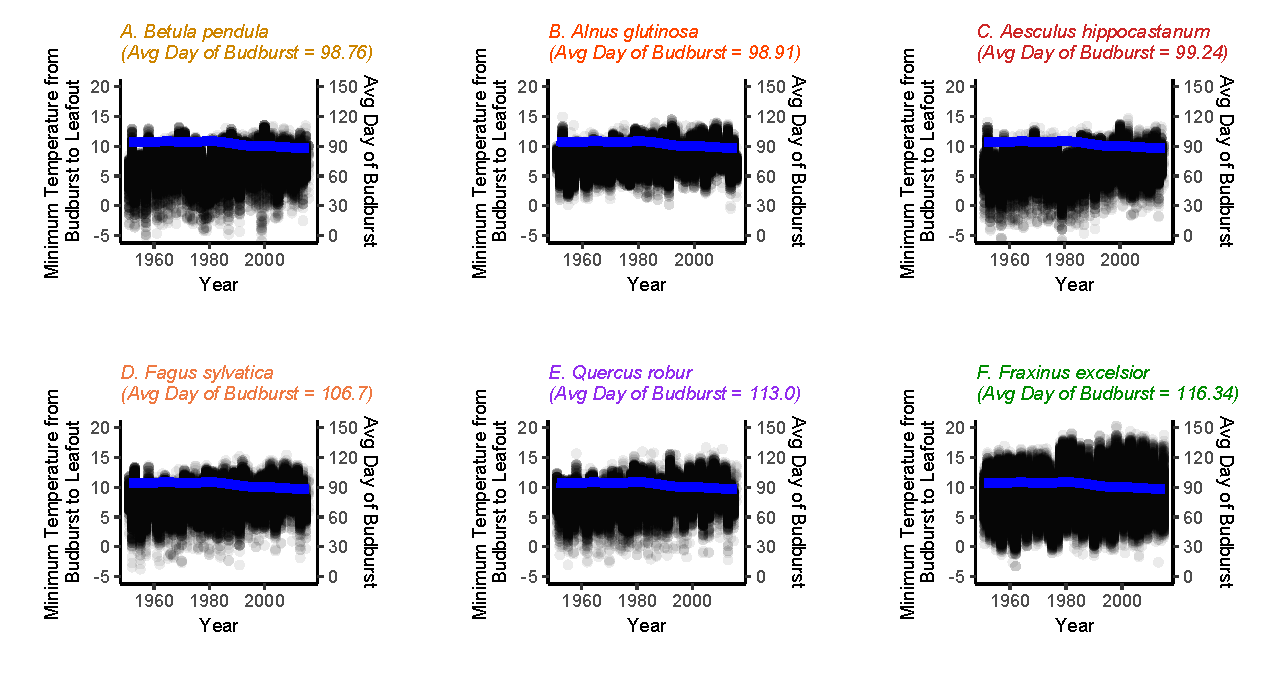
\includegraphics[width=16cm]{..//figures/TminBB_bySpp.png}
  -\caption{Minimum temperatures between budburst and leafout are plotted for each site over time (from 1951-2016) for each species. The blue line is a smoothing spline, indicating the trend of average day of budburst for each year for each species. Species are ordered by average day of budburst, with the earliest being \textit{Betula pendula} and the latest being \textit{Fraxinus excelsior}. }\label{fig:tmin}
  -\end{center}
  -\end{figure}}
  
  {\begin{figure} [H]
  -\begin{center}
  -\includegraphics[width=12cm]{..//figures/model_output_dvr_50.pdf}
  -\caption{Model output with different durations of vegetative risk for each species. More positive parameter effects indicate an increased probability of a false spring whereas more negative effects suggest a lower probability of a false spring. Uncertainly intervals are at 50\%. Parameter effects closer to zero have less of an effect on false springs. There were 744,295 zeros and 10,491 ones for false spring in the data.}\label{fig:dvr}
  -\end{center}
  -\end{figure}}

{\begin{figure} [H]
  -\begin{center}
  -\includegraphics[width=12cm]{..//figures/model_output_berniefive_50.pdf}
  -\caption{Model output with a lower temperature threshold (-5$^{\circ}$C) for defining a false spring. More positive parameter effects indicate an increased probability of a false spring whereas more negative effects suggest a lower probability of a false spring. Uncertainly intervals are at 50\%. Parameter effects closer to zero have less of an effect on false springs. There were 755,677 zeros and 1,025 ones for false spring in the data, rendering a less stable model.}\label{fig:five}
  -\end{center}
  -\end{figure}}
  

%{\begin{figure} [H]
%  -\begin{center}
%  -\includegraphics[width=16cm]{..//figures/PropSitesbyYrwBB.png}
%  -\caption{The black line indicates the proportion of sites that had false spring conditions for each year across all species. The blue line is a smoothing spline, indicating the trend of average day of budburst for each year for each species. Species are ordered by average day of budburst, with the earliest being \textit{Betula pendula} and the latest being \textit{Fraxinus excelsior}.}\label{fig:fsprop}
%  -\end{center}
%  -\end{figure}}

\end{document}
